% Chapter 4
\chapter{Advertisement decision} % Main chapter title

\label{Chapter4} % For referencing the chapter elsewhere, use \ref{Chapter1} 

\section{Introduction}

At the time of industrialization, industries compete on product quality, and modern organizations focused more on delivering services, and now services and products is hardly able to be distinguished because of they provide various offers and consumers lose themselves in it, as Peter van Waart describes in his paper that ``\emph{In the last two decades however, economical developments resulted in the experience economy: a new era of marketing and branding, in which traditional advertising is becoming less effective and meaningful experience branding is key}'', \cite{Meaningful_ad}, therefor economical developments have changed from time to time and is emerging from economical experience and factors like price-reduction for a brand is not so important, but experience factor has become the central part for the development.Any advertisement that explains a product features and why that matters fails to achieve people satisfaction, because people’s experience were not considered in it, as Joško Brakus \cite{Brand_experience} explains the measurement of brand experience and how it can effect on product loyalty.\\

Now at this era where the technology is highly advanced and most people especially youngsters are much familiar with them like using smartphones, Tablets and now even wearable computers like Apple watch, and also there are many developments in sensing technologies like body tracking, hand recognition, By using these technologies different interactions are possible and very attractive and funny interactive advertisement can be developed so that could engage more participants.\\

As a computer scientist, there had been no chance to create an advertisement but have always been interested in advertisements; Advertisements are always unique and attractive to watch, at least for the first time. Therefor there is a need to conduct a study with the people who have been working in advertisements for long time and have experience and professionalism in related domain. The people working for Bauhaus-Walk as tour guides understands much more about the topic than anyone else, because they run the program, know tourists, understand tourist's Interests and many more.\\

Focus group methodology has been selected to have more insight on the deciding an Interactive Advertisement for the Bauhaus-Walk program. Focus group is a small group usually between six up to ten participants joint together in comfortable place usually a quite room, to discuss on a specific topic domain and share ideas. As described by Jenny Cameron ``\emph{Focus groups can be exhilarating and exciting, with people responding to the ideas and viewpoints expressed by others, and introducing you, the researcher, and other group members to new ways of thinking about an issue or topic }''\cite{FocusGroup}.As Florian Alt \cite{mobile_focus_group}talks about the process of how the focus group was conducted for a mobile contextual display systems. \\

Focus group was conducted to get more detailed information about Bauhaus-Walk program and its content. This was mainly meant to understand many aspects of Bauhaus-Walk and collect the required parameters for designing the interactive advertisement. Because of time limitation in each session two sessions were arranged in two different dates to cover all topics and discussions. This chapter describes the main theme and goal for focus group and reports all the processes that were taken to establish the focus group, how participants were invited and what was being discussed and more focused on each session. How data was gathered and what techniques were used to analyze them. The document presents all the findings and outcomes in details and related discussions and conclusions.\\

\section{Research Questions}
To design the interactive application advertisement it was required to collect the bellow information from the Bauhaus-Walk members. So that we develop a very relevant advertisement that could speak by itself for Bauhaus-walk program and at the same time it should be entertaining and funny for the passers-by that want to play with advertisement and remember the experience for long time and as a result be motivated to take the tour. Therefor we would need to understand many aspect of Bauhaus-walk as listed bellow in short.

\begin{enumerate}
\item Who is (are) the target Group?
\item What are the existing Bauhaus-Walk advertisement medium?
\item What are the peak times in the year for Bauhaus-walk tour?
\item Which are the tour routes?
\item Which famous Locations are included in the tour?
\item What are important aspects of Bauhaus-Walk from their point of view?
\item What could be a suitable interactive advertisement theme?
\item Which content should be in advertisement?
\item What engagement techniques should be integrated in advertisement?
\item What kind of advertisement would be suitable for both body and mobile techniques?
\end{enumerate}

\section{Study design}
Focus group was designed in two sessions mainly because of the participants could not be present all at the same time or date, and by doing we also had enough time to analyze the first session and discuss the findings in the second session with new participants and get their point of view, the first session was more related to gathering general information about Bauhaus-Walk program and second session was more in depth discussions on the advertisement decisions. 

\subsection{Participants}
The focus group in this study consists of six participants including the Moderator, which will be me (Hasibullah Sahibzada). They will be divided in sub groups based on their professionalism, position to be able to discuss among each other comfortably, if possible or will be considered as only one group for discussions.
The participants were invited through doodle, where a varieties of date slots are available to select, and can see other participants joining time and date. A short introduction of the focus group was described in. The complete focus group session lasted about 90 minutes

\subsection{Focus-Group Environment}
The focus Group was held inside the DBL building ground floor, where we had enough space to make a group circle. Participants were offered coffee and biscuits at the beginning or end of the session.


\begin{figure}[H]
    \centering
    \subfloat[]{{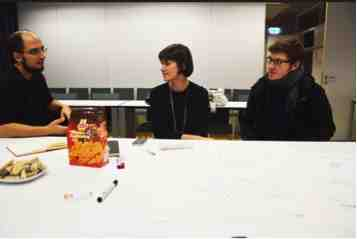
\includegraphics[width=6cm,height=4cm]{Figures/4/focus_group} }}%
    \subfloat[]{{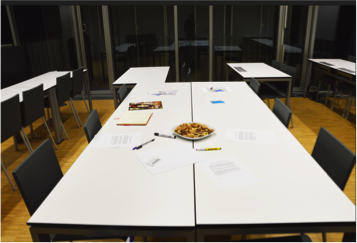
\includegraphics[width=6cm,height=4cm]{Figures/4/meeting_room} }}%
    \caption{A: Focus group. B: DBL meeting room.}%
    \label{fig:Focus_group_room}%
\end{figure}


\subsection{First session}
This session was an exploratory session for Bauhaus-Walk program, and a good start for us to think different domains about interactive advertisements.

\subsubsection{Questions}
\begin{enumerate}
\item   What kinds of advertisements for Bauhaus-Walk are there?
\item   Who join the Bauhaus-Walk program in general?
\item   What could be a suitable theme of Bauhaus-Walk for the Interactive advertisement?
\item   What would be the content of the advertisement?
\item   How to motivate passer-by to be engaged with the advertisement?
\item   How to engage passers-by with the advertisement?
\item   What kind of Gesture and Mobile Interactions should be used?
\item   How to motivate passer-by to join the actual Bauhaus-Walk tour?
\item   Is there anything else we need to discuss on Bauhaus-Walk Advertisement? Any new angle?

\end{enumerate}

\subsubsection{Procedures}
Participants were warmly welcomed and asked to feel comfortable by having biscuits and coffee. I introduced myself and asked them to introduce themselves. This helped to understand each others professional background and interests. 

\begin{enumerate}
\item Introduction \\
Brief introduction on advertisement and interactive advertisements were given to participants to understand the possibilities of existing technologies and the use of them in advertisement field. Some interactive advertisements were introduced with their relative interaction techniques. The agenda and goal of thesis was also described to have a wide picture of what is going to be done till the end of this semester.


\item Discussion session \\
After introduction, discussion started on bellow mentioned questions. Because there was limited number of participants I could not divide them in to groups to discuss in detail and do comparative study among the groups. They were given sheet empty big papers to draw and write what come in their mind while discussing to be able to keep track of their thoughts and be easy to generalize the opinions. During the discussion Patrick Tobias Fischer was asked to write notes on the discussion.

\item Consent Form \\
Each participant was asked to sign the consent form to make sure they agree to participate and video recorded.

\end{enumerate}


I was responsible to carry on the entire discussion and Patrick Tobias Fischer was doing the note taking during the discussion. He noted important information extracted from our discussions so that I could later look at them beside that the entire discussion was also video recorded for analyzing.


\begin{figure}[H]
    \centering
    \subfloat[]{{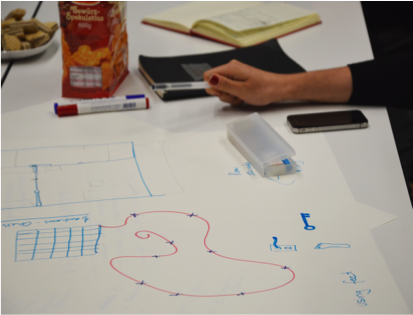
\includegraphics[width=6cm, height=5cm]{Figures/4/drawings} }}%
    \subfloat[]{{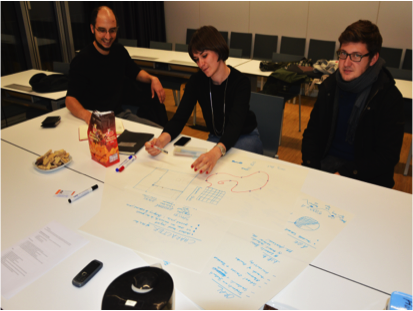
\includegraphics[width=6cm, height=5cm]{Figures/4/discussions} }}%
    \caption{A: Drawing information in to sketches B: Group discussion. }%
    \label{fig:observation_env}%
\end{figure}


\begin{figure}[H]
    \centering
    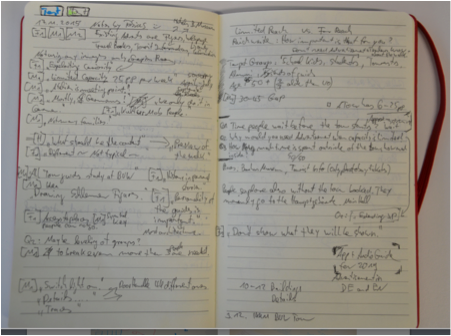
\includegraphics[width=6cm, height=5cm]{Figures/4/notes}%
    \caption{Observation notes}%
    \label{fig:observation_note}%
\end{figure}


\subsection{Second Session}
Based on the first focus group's discussions and the participant's nice ideas, which are mentioned in finding section, two different paper prototypes of advertisement were made to dig more in detail. The participants were given the prototypes to play with them and explore their own way of designing the advertisement and interaction.

First prototype was Bauhaus-Chess, This prototype was chosen because of the historical background of this amazing chess game that was developed by Josef Hartwig \cite{Josef} long time before. The shape of the chess piece defines the movement direction of itself on the chessboard. The goal was to show the chess on the advertisement screen and show one piece at a moment and let users to move the chess in the right direction by some sort of gesture. 

Second prototype was to show map on the screen and possible interactive famous places, the interaction idea was to map physical movement of a person to the virtual movement inside the advertisement and let them to explore the target places by reaching their silhouettes on them. Maximum three places were to be explored by one person.

The basic ideas were designed to help the participants to think more and come up with some more ideas and at the same time should be in the context of Bauhaus-Walk program. 

\subsubsection{Procedures}
\begin{enumerate}
\item   Short introduction was given on Interactive Advertisement thesis.
\item	Short motivational video of interactive advertisement was shown.
\item	Two paper prototypes that are mentioned above (Bauhaus chess and Map) were introduced.
\item	Possible interactions were shown to them.
\item	Participants were asked to comment on prototypes and come up with new ideas and interactions.
\item	They were asked to design their own prototype.
\item	Integrate some fun ideas with prototypes.
\item	What contents should be included in the prototypes.
\item	How to gather and collect those contents.
\end{enumerate}

\subsubsection{Prototype and discussion pictures}

\begin{figure}[H]
    \centering
    \subfloat[]{{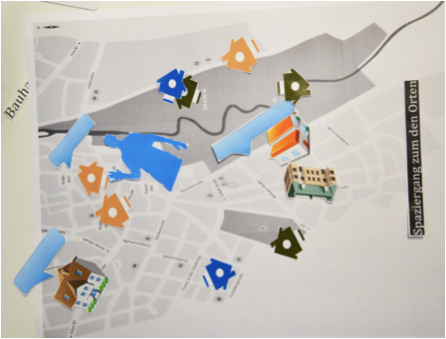
\includegraphics[width=6cm, height=5cm]{Figures/4/map} }}%
    \subfloat[]{{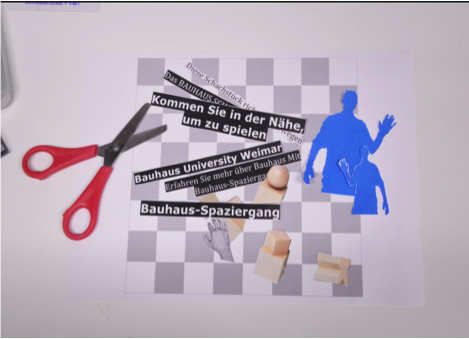
\includegraphics[width=6cm, height=5cm]{Figures/4/chess} }}%
    \caption{A: Map prototype, B: Chess prototype }%
    \label{fig:observation_env}%
\end{figure}


\begin{figure}[H]
    \centering
    \subfloat[]{{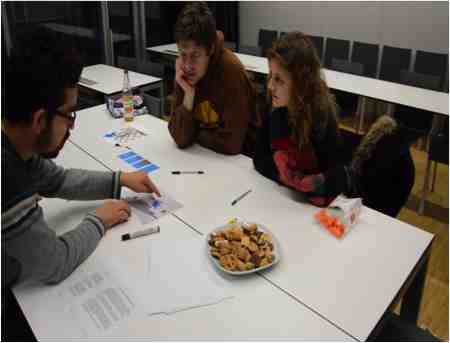
\includegraphics[width=6cm, height=5cm]{Figures/4/show_map} }}%
    \subfloat[]{{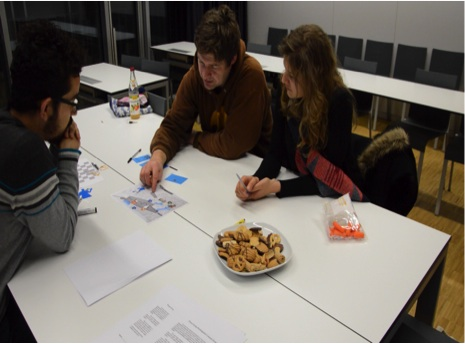
\includegraphics[width=6cm, height=5cm]{Figures/4/tell_map} }}%
    \caption{Explaining and discussions on prototypes }%
    \label{fig:observation_env}%
\end{figure}


\subsection{Data Gathering}
The entire session was video recorded for analysing. Note taking technique was used to write down the major and important parts of the discussions.Beside the noted taking we encouraged the participants to discuss the issues on a piece of chart using drawings and texts, this helped the participants to focus on their ideas and build the ideas in a more better way and at the same time that helped us to have a summary of their opinions and thoughts. Photos were also taken from the participant while discussing ideas and from the skitches they drew. Check Appendix \ref{AppendixB}


\section{Findings}
The design of this focus group was done in a way that could be very easy to be analyzed and generalized in very little amount of time. 

\begin {itemize}
\item	Participants were asked to draw sketches and write on the given big sheets of paper on the topics they were discussing.
\item	They could make summary of their discussion on the paper so that they and we fully understand the topics.
\item	Tobias Patrick was taking notes to cover up everything we discussed.
\item	All the sessions were video recorded for full detailed analyzing. 
\end{itemize}

All of the above resources were analyzed by going through each of the sketches they drew and each notes that were written and all the videos were seen many times to check if some ideas were not clear in the sketches or notes and to have a final image of the discussions.



\subsection {First Session Findings}
The bellow sections are extracted from the long discussions, and analyzing video and drawn charts.


\subsubsection{Reason of Bauhaus-Walk and advertisement}
Bauhaus-Walk is a project that is run by university students to show more about Weimar and Bauhaus culture to the world by giving small tours to group of maximum 30 people. The tour shows studying conditions of the university and students, living style of people and giving excursion to historical places.

Guides are from different backgrounds like architecture, urbanism and design and each of them could show various aspect of Bauhaus by their own stories and inter-relate the stories with the facts and then connect them to the places in Weimar. Most important for the guides are not just the buildings but also the small details inside the building that most people do not focus, guides want to be the voice of those unspoken stories for the tourists.

Current existing advertisements for Bauhaus Walk is through different mean as listed bellow.

\begin {enumerate}

\item	Web
Bauhaus Walk is advertised briefly in the Bauhaus University Weimar webpage \cite{Tourist_info} and in Weimar tourist information page \cite{Bauhaus_Walk_Uni}

\item	Print
Bauhaus Walk program are advertised in flyers and leaflets at different locations, like they could be found in tourist information center, Bauhaus Museum, calendar of Weimar and in travel leaflets. 

\item	Books
Bauhaus Encyclopedia has mentioned this program too. 

\item	Oral
Mostly the people who have already taken the program once publicize it and they let their friends, relatives and family know about it.


\end{enumerate}

As stated above Bauhaus-Walk already has many ways of advertising and at the same time an the making of interactive advertisement was proposed by me there are many reasons that why Bauhaus-Walk would need advertisement as stated bellow.


\begin {itemize}
\item   Extend the current situation.
\item	Create new audience.
\item	Get more people on regular basis.
\end{itemize}


\subsubsection{Target group}

Most of the people who join the tour are from elder people ranged between 45-65 years old and others are adults and children. Adults mostly learn about the program trough web and the elders learn from the tourist information centers and books.  Most of the participants are German and do not understand English language.

\begin{figure}[H]
    \centering
    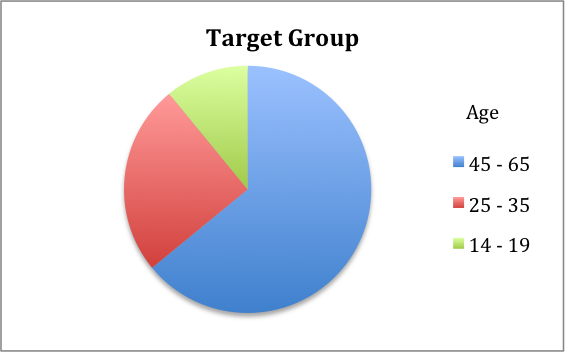
\includegraphics[width=6cm]{Figures/4/target_group}%
    \caption{Target Group}%
    \label{fig:target_group}%
\end{figure}


\subsubsection{Peak Tour times}
In Average 5000 people take the tour each year. April, May, September and October are the peak months that people take the tour because of the weather condition to be good the amount of people per tour is about 25 people, but in winter there are very few people joining the tour and the amount of people per tour is up to five to six. 

\subsubsection{Possible advertisement location}

\begin {enumerate}

\item	Tourist Information. \\
This is a good place to put Bauhaus-Walk advertisement because 
\begin {itemize}
\item	Random visitors from different places and cities come here and want to know about Weimar in general. 
\item	Heavy traffic of people.
\item	This is the only place to get Bauhaus-Walk tickets in advance.
\end{itemize}


\item	Bauhaus Museum. \\
This could be another good place, but people have to pay to enter to this museum, so there will be limited people but who
\begin {itemize}
\item	Are very interested in Bauhaus.
\item	Likely to go on tours.
\end{itemize}


\item	University main building. \\
Main university building is a more open place for all visitors; there are many factors as stated bellow.

\begin {itemize}
\item	People from different background.	
\item	People from different age, more youngsters like students.
\item	Interested people in Bauhaus.
\item	It is close to starting point of Bauhaus-Walk tour.
\end{itemize}


\end{enumerate}


\subsubsection{Content of advertisement}
Participants pointed on very important thing about the content of advertisement from which the advertisement got clearer and clearer and could be categorized in to many different aspects of Bauhaus-Walk.


\begin {enumerate}

\item	Objects \\
There are objects that are introduced during the tour for the tourists; A good idea would be to show those objects on various locations on the map that they belong to.
\item	Stories \\
Bauhaus Walk tour guides have many stories to tell about the walk and their own backgrounds as one of them said ``\emph{Probably our walk is to sum it up, consists of stories we are actually telling stories, not just talking about history, not just about facts but our own personal stories and stories that were told by former students, so we are kind of raping the history in to personal stories, and we want to say that hay, we are students from different faculties and we want to tell the stories by different ways, and that is not a bad thing, because based on historical fact that there has not been the same Bauhaus in Weimar, there has been so many different teachers and students and they all had a different idea that what Bauhaus could be and I think we still kind of incorporate that the fact that no Bauhaus tour would be the exactly the same like the others before.}''
\item	Histories, Facts, Places

\end{enumerate}

\subsubsection{Interaction of advertisement}
Based on the examples that were shown at the introduction for the participants, they like hand gesture and some other and came to the bellow possible techniques.

\begin {enumerate}
\item	Hand gesture Interaction. \\
The bellow two kinds of interactions were discussed each containing different contents. 

\begin {itemize}
\item	Hovering: \\
By showing the Bauhaus map on the screen with the most important elements on it, the users should be able to look at the items by moving their hands on top of it. The items could change its status when hovering for example if there is a light object shown by hovering it should turn on or something like that.
There could be famous places shown on the map that Bauhaus-Walk tour focuses most, and by hovering the hand some more information like a picture or a related to that places should be shown.

\item	Performing a specific gesture:\\
There are many objects that have specific characteristics and thso details are described in the tour, so the idea was to bring those object in action and allow users to perform those actions, one idea was to show a 3D environment and the user should be able to perform a gesture like opening door handle, lighting up a lamp, opening a lock by a key or play with Bauhaus SCHACHSPIEL chessboard to navigate the correct movement of the chess piece on to the screen, or other different gestures for specific tasks.

\end{itemize}

\item	Body Interaction  \\
Bauhaus-Walk is known from its name that it is all about walking to different historical places therefor there was the idea of giving short virtual walk on the screen by moving the user's body in front of the screen and exploring some sights.

\end{enumerate}


\subsection{Second Session Findings}
The second session was held after a week and half, with only two participants other participants could not come because they were busy with their studies. 

\subsubsection{Prototype discussion}
Participants understood both prototypes along with their mobile interactions concept, and liked both prototypes in terms of interaction and idea. And commented as bellow. I categorized their comments in two positive and negative sections as bellow.
\begin {enumerate}

\item Chess-Game

\begin {itemize}

\item{Positive points:} 

\begin {itemize}
\item	The idea is very nice, because many of the visitors are above the age of 40 and they may be familiar with this game.
\item	Easily understandable by looking at the shape, because shape defines the movement. 
\item	Suites best for Bauhaus Museum because, there is the original chess board of Bauhaus but people are not allowed to touch the game, by bringing this type of interaction, people will have a live experience with the chess board and play around with it and understand it.

\end {itemize}

\item{Negative points:} \
\begin {itemize}
\item	Very difficult to understand by people who have not played chess before or have not seen this special type of chess.
\item	Players could make a lot of mistakes while moving the chess piece. 
\item	The idea does not really fit to the Bauhaus-Walk program.
\item	It does not fit the places that are being shown in the tour.
\end {itemize}
\end {itemize}

\item Map-Game 

\begin {itemize}

\item{Positive points:} 
\begin {itemize}

\item	Map game idea fits a lot to Bauhaus-Walk tour.
\item	Portraits the idea of walking by body interaction.
\item	Easy interaction just by moving body and navigate inside the screen.
\item	Understandable concept by moving on to different places and exploring them. 
\end {itemize}

\item{Negative points}
\begin {itemize}
\item	Possible moving difficulties in a given space.

\end {itemize}
\end {itemize}
\end {enumerate}

Based on the discussions, the Map-Game was accepted for further discussion and Chess-Game was exploded for further discussion because of the crucial negative points.


\subsection{New ideas}
\begin {itemize}

\item	Content of the game should be very clear and accurate and they should show the places where we provide tour. We do not have many places to show and there may be maximum three places.
\item	Integrating some fun factor to the game and interaction like by showing a famous character face on top of the silhouette head position. And giving a kind of funny movement. 
\item	Giving opportunity for multiusers to play interactive game, like for example if there are two people standing in front of the screen, the tasks will be divided among them by locking one's silhouette or interaction and allowing the other to perform the task.
\item	Defining the task by the defined character or by color of the body or by random. 
\item	Showing funny map, which was made many years back of Weimar city.
\item	Popping up interactive objects (houses) on the screen so the users understand that they are interactive. 

\end {itemize}


\section{Conclusion}
The conduct of the two sessions of focus group was very helpful in a way that it was held very intensive that helped to understand in general the whole about Bauhaus-Walk program tour and especially about the tour guides that what they think about Bauhaus-Walk and what are the most important things that could be discussed and advertised for Bauhaus-Walk. All the relevant mentioned questions for the design and interaction of advertisement were answered and discussed. As a result of this focus group, one interactive advertisement prototype would be purposed, that should be able to cover all the aspects of advertisement and concept of Bauhaus-Walk that was discussed in this focus group and the findings from attraction attention and last from findings from people interviews.
